\documentclass{article}

\usepackage{amssymb}
\usepackage{amsmath}
\usepackage{graphicx}
\usepackage{epsfig}
\usepackage{subfigure}
\usepackage{listings}
\usepackage{natbib}
\usepackage{verbatim}
\usepackage[T1]{fontenc} 
\usepackage[hyphens]{url}
\usepackage{stmaryrd}
\lstset{language=ml}
\lstset{commentstyle=\textit}
\lstset{mathescape=true}
\lstset{backgroundcolor=,rulecolor=}
\lstset{frame=single}
\lstset{breaklines=true}
\lstset{basicstyle=\ttfamily}

\begin{document}

\title{Query languages applied to game development}

\author{
\textbf{Giuseppe Maggiore} \and \textbf{Giulia Costantini} \\
       Universit\`a Ca' Foscari Venezia\\
       Dipartimento di Scienze Ambientali,\\
       Informatica e Statistica\\
       \texttt{\{maggiore,costantini\}@dais.unive.it}
}

\date{\today}
\maketitle

\begin{abstract}
In this report we summarize the application of declarative query languages to game development. Thanks to the use of a language that is very similar to SQL the authors have been able to build games with complex logic, fast runtime and very little and easily readable code.
\end{abstract}

\section{Introduction}
\label{sec:intro}
%%%%%%%%%%%%%%%%%%%%%%%%%%%%%%%%%%%%%%%%%%%%%%%%%%%%%%%%%%
% intro.tex
%%%%%%%%%%%%%%%%%%%%%%%%%%%%%%%%%%%%%%%%%%%%%%%%%%%%%%%%%%


\begin{figure}
\begin{center}
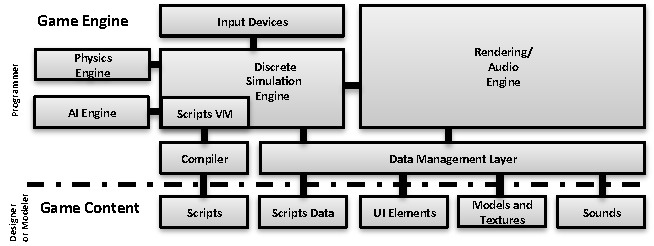
\includegraphics[scale=0.8]{engine_architecture.pdf}
\end{center}
\label{fig:data_driven_games}
\caption{Data-driven engine architecture, from \cite{SGL}}
\end{figure}

Virtual reality browsers face big challenges centered on performance and complexity. Performance is needed because the framerate at which the virtual world is rendered and animated must be high enough to give the user a feeling of smoothness. The scene must be rendered at least at 30 frames per seconds, but higher framerates (e.g. 60 frames per second) are perceived by the user as more pleasant.

Both the visual and logical complexities of a virtual world are very important. Visual richness gives the user the impression of a more realistic and detailed world, with many beautifully rendered objects, while logical complexity permits articulated responses that give the user the feeling of being part of a realistic world with its own set of rules and internal laws.

One of the most important tasks for developers of interactive worlds is to find the right trade-off between these sometimes conflicting requirements. Increasing performance requires a mixture of compromise (reducing the size of the world or ``dumbing down'' its responses) and time-consuming low-level optimization. We believe that automated optimization of interactive applications is a fundamental frontier if we wish to enable developers to build richer worlds without exponentially increasing costs.

Modern 3D browsers and engines are based on a data-driven architecture as shown in Figure \ref{fig:data_driven_games}, taken from \cite{SGL}.

In a data-driven engine the engine contains only general knowledge about virtual worlds, but nothing specific about the peculiar features of a specific virtual world. The specific virtual world will be loaded from the game content in the form of configuration files and scripts. A data-driven engine loads from files two main datasets:

\begin{itemize}
\addtolength{\itemsep}{-0.5\baselineskip}
\item a \textbf{scene}, the set of entities that populate the virtual world
\item \textbf{scripts}, the set of (possibly complex) behaviors that animate the scene entities
\end{itemize}

The scene is composed by a heterogeneous set of entities, each of a different kind. Entities may be virtual characters, trees, 2d or 3d models; entities may also be purely logical and invisible entities such as timers, triggers and proximity sensors.

Scripts give depth to a scene by implementing complex interrelationships between entities. Scripting can be done at three different levels of increasing complexity and expressive power:

\begin{itemize}
\addtolength{\itemsep}{-0.5\baselineskip}
\item \textit{routing} is a simple transmission of values from one entity to another
\item more complex scripts can perform data conversions when moving information between entities
\item even more advanced scripts can create, remove or modify entities of a scene
\end{itemize}

The usual implementation of an engine (see \cite{GAME_OO_HIERARCHY}) features an object-oriented architecture of classes. At the root of this architecture is a class that represents the most generic entity, and from which all other entities are derived. The engine maintains a list of these generic entities, which are all updated and handled through a set of virtual functions. This architecture is a source of often underestimated overhead. Dynamic dispatching is not too costly for a few calls, but when we have many entities, the cost of invoking various virtual functions many times for each frame can become very high. Sometimes the cost of the dynamic dispatching architecture may become higher than the cost of the actual operations being dispatched.

Scripts usually access the scene dynamically. This means that a script must look for the right entities with a mixture of lookups by name and unsafe casts. For example, consider how a Java script may access the \texttt{time} field of a \texttt{myClock} node of type \texttt{timer}:

\begin{lstlisting}
\addtolength{\itemsep}{-0.5\baselineskip}
X3DNode myClock = 
 mainScene.getNamedNode("myClock");
SFTime time = 
  (SFTime) myClock.getField("time");
\end{lstlisting}

This style is unsafe, since \texttt{myClock} may not exist or it may have the wrong type, and it also incurs in significant overhead.

In this paper we will focus exclusively on the X3D language, since it is a recognized standard and it offers a good benchmark to test virtual worlds where we can specify our scene and its various scripts. In the paper we show how we have tackled the problem of increasing performance in X3D browsers while also making scripts safe. We have used a simple compilation technique that removes many unnecessary dynamically dispatched invocations; this technique also allows us to introduce safety for scripts that access the state, so that they do not need to perform unsafe dynamic lookups when searching for specific nodes. To the best of our knowledge, this is the first approach that experiments with compiling X3D scripts and scenes in order to achieve greater performance and safe scripts. None of the previous approaches we are aware of focuses on compilation of X3D as a means to achieve both higher performance (by reducing overhead) and safety (by introducing compile-time checks). Higher performance through compilation includes a long list of research work such as \cite{OPT1,OPT2,OPT3} which has shown that compilation can yield better runtime performance by reducing dynamic overhead and improving other properties of the generated code. Similarly, introducing safety in dynamic languages such as scripting systems has been studied in general in the context of generating typed programs from untyped scripts in \cite{SAFESCRIPTS1}, and the problem of statically typing information which is generally untyped has also been explored in the Haskell community in \cite{SAFESCRIPTS2} among many others.

In Section \ref{sec:solution_workflow} we discuss the general architecture of our system. In Section \ref{sec:compiling_scene} we show how our technique generates the code and the type definitions that represent a scene. In Section \ref{sec:case_study} we show an example of a compiled scene and its routes. In Section \ref{sec:benchmarks} we report some benchmarks that show speed increasing when rendering a sample scene with just nodes and routes by applying our technique. Finally, in Section \ref{sec:compiling_scripts} we discuss how we represent scripts that externally access the scene.

 

\section{Data-driven games}
\label{sec:ddg}
%
% ddg.tex
%

A data-driven game \cite{10} separates game content from the game code. This design allows both game programmers and game designers (groups with very different skillsets) to contribute separately to game development. This separation has long been practiced, for example by storing models, textures and sounds in data files separate from the game engine; this trend has recently accelerated by trying to move as much content as possible out of the engine: character and story-line data is increasingly \cite{25} being stored in external configuration files. Modern design goes even further, storing game logic specific to game play in external files written in a scripting language such as Lua, Python or a custom-made scripting language \cite{SCRIPTING_LUA,SCRIPTING_PYTHON,UNREALSCRIPT_LATENT_FUNCTIONS}.

\begin{figure*}
\begin{center}
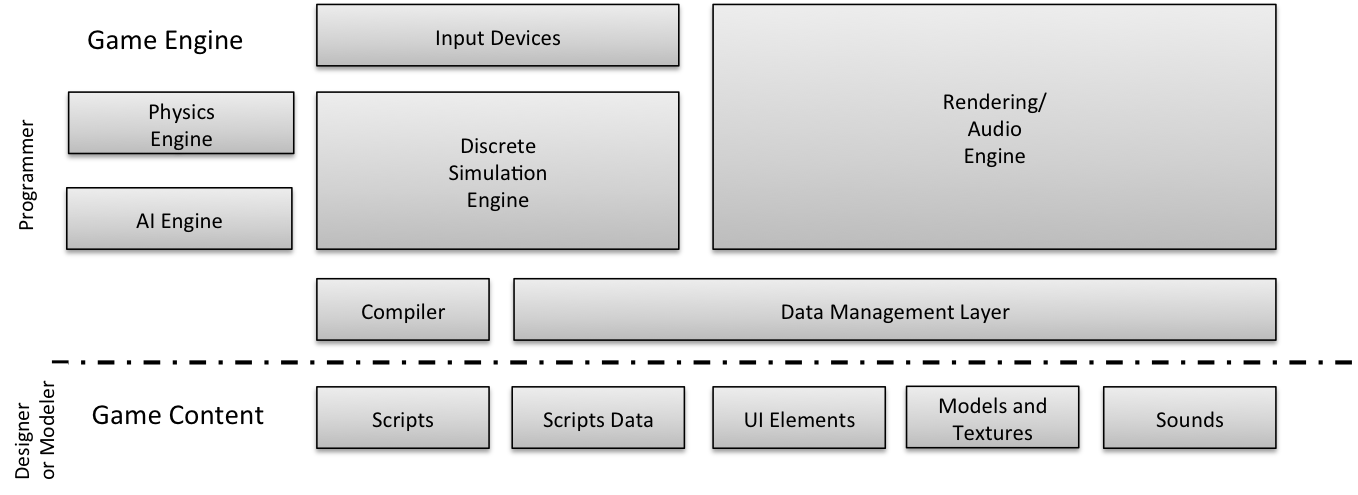
\includegraphics[scale=0.5]{engine_architecture.png}
\end{center}
\label{fig:data_driven_games}
\caption{Data-driven game architecture}
\end{figure*}

In Figure 2 we can see the general architecture of a data-driven game. The game engine (AI, physics, rendering, audio and discrete simulation) is written and maintained by programmers. Typically, the discrete simulation engine puts together the interactions between physics, AI and game logic in a meaningful way, and exposes the resulting game state and events to the rendering and audio engine which give some feedback to the player. The game content is created by game designers, who are responsible with creating and populating the game world; the game world contains both artistic elements like models and sounds, but also logical elements such as behaviors and character statistics. Logical elements are defined by scripts; scripts are either compiled or interpreted and executed by the discrete simulation engine. Separating scripts becomes important in all those game where character behavior must be tested and adjusted constantly during development to ensure that there is no single optimal strategy that can ensure victory (otherwise the game would lose much of its challenge and interest). Also, separating game logic into scripts allows for ``modding'', that is players can modify the game even without access to its source code; the creativity of the players can extend the lifetime of a game beyond the original intentions of its developers (\cite{21}). The entire focus of the authors is on the discrete simulation engine and how techniques taken from the database comunity can be used to build a better performing implementation that can be heavily scripted.

\paragraph{The Discrete Simulation Engine}
Game are processed in clock ticks. During each clock tick the simulation engine processes the current state of the world, thereby computing its updated version. This usually consists in considering the actions of all the characters of the game (some characters may perform null actions, but still they are given an opportunity at every tick); each action may produce several \textit{effects}.  Effects produced during the same tick are written into the game state simultaneously, allowing us to cleanly separate each clock tick into three stages:

\begin{itemize}
\item a query stage when we read the contents of the game data
\item a decision stage where we choose the actions of each character
\item an update stage where we write into the game state the effects produced by each action
\end{itemize}

Since actions are all updating the game data simultaneously, we use a transaction model to describe how these updates are processed. Since effects usually increase or decrease numeric values then such a model becomes simply an aggregate function such as \texttt{(+), (-), max, min, ...}. Effects are usually separated into \textit{stackable} and \textit{non-stackable}, depending on whether or not they accumulate during one tick or only one update is picked; for example, damage is stackable since a unit that suffers damage from multiple opponents receives the sum of all these damages, while healing auras are non-stackable because only the most beneficial aura is applied while all the others are discarded.

\section{Real-time strategy games}
\label{sec:rts}
%
% rts.tex
%

Real-time strategy games are the ideal field of application of techniques that increase the number of supported characters, as demonstrated by the number of units available. In these games, the player controls large numbers of \textit{units} which are selected and which receive commands; the execution of commands by each unit is controlled by the AI; the smarter the AI, the more entertaining the game: a player wants his units to follow his instructions correctly, without having to specify too many details; this way, when the player has issued orders to some units, he can move to other portions of the map and give other orders to other units while the original orders are being carried out. Unfortunately unit behavior in current RTSes is quite primitive, usually modeled with simple finite state machines. As a result, players need to issue many orders to achieve a good level of coordination between his units. Processing scripts that handle the correct behavior of each unit is very expensive at run-time, since each unit is typically processed separately. A typical solution to this problem is that of processing units in groups (centralized AI); with this technique each script controls a large number of units, which then behave with good coordination. For example, in the game \textit{Warcraft III}, the AI for each computer player is divided in two commanders: defence and attack. Centralized AI often has problems when trying to maintain actions over multiple fronts (more than the number of virtual commanders available), and it is of no help to the human player. Having smarter units would benefit both the computer player and the human player.

Note that centralized AI is just an ad-hoc form of set-at-a-time processing, explicitly implemented by the game designer who aggregates units knowing that they will perform a similar role. The authors propose to build a scripting language that makes grouping units behaviors together more systematic with a declarative language like SQL, paired with a set of optimizations appropriate for games.

The most important functionality of scripts will thus be implemented with a purely functional language with aggregate operations on sets. The case study will be a synthetic RTS with three types of units:

\begin{itemize}
\item armored \textbf{knights} who can move and attack at short range
\item \textbf{archers} who can move and attack at long range
\item \textbf{healers} who heal friendly units within a certain range; healing auras are nonstackable
\end{itemize}



% syntax, semantics (informal), optimization (informal)
\section{SGL}
\label{sec:sgl}
%
% sgl.tex
%

Game data is modeled as a relation $E$. This table is a multiset and it needs not have keys. Each row in the table represents a unit or object, with information such as health, speed, damage, special properties, etc. Each row also contains data representing messages to this unit, such as data coming from the pathfinding system, cooldown periods, and so on. One possible definition of $E$ for our example could be:

\begin{lstlisting}
E(key,player,posx,posy,health,cooldown,
  weaponused,movevect_x,movevect_y,damage,inaura)
\end{lstlisting}

The attributes \texttt{key ... cooldown} represent the state of the unit; these attributes are not modified directly from a script, but rather they are modified accordingly to the values of \texttt{weaponused ... inaura}, which represent the effects that unit is being subjected to.

An SGL script consists of a single action for a single unit, and at each tick it will be executed and it will take an entire environment $E$ and it will return a new environment $E_u$. All environments $E_u$ are then combined into a single environment in which the effects are applied with a post-processing step. A possible post-processing related to the schema above could be (where \texttt{norm} normalizes movement velocity):

\begin{lstlisting}
SELECT u.key, u.player, 
       u.posx + u.movevect_x * norm AS posx, 
       u.posy + u.movevect_y * norm AS posy, 
       u.health - u.damage + u.inaura AS health, 
       u.cooldown - 1 + u.weaponused*_TIME_RELOAD AS cooldown, 
       0 AS weaponused, 
       0 AS movevect_x, 
       0 AS movevect_y, 
       0 AS damage, 
       0 AS inaura
FROM E u 
WHERE u.health > 0
\end{lstlisting}

The post-processing step above applies the effects to the state and resets the effects to avoid applying them again during the next time step.

\paragraph{Syntax of SGL}
SGL scripts have a simple syntax consisting of a mix of ML (\texttt{let, if-then-else}) and SQL:

\begin{lstlisting}
main(u) { 
  (let c = CountEnemiesInRange(u,u.range)) 
  (let away_vector = (u.posx, u.posy) -
         CentroidOfEnemyUnits(u, u.range)) { 
           if (c > u.morale) then
             perform MoveInDirection(u,away_vector); 
           else if (c > 0 and u.cooldown = 0) then
             (let target_key = getNearestEnemy(u).key) { 
             perform FireAt(u, target_key);
} } }
\end{lstlisting}

Where the auxiliary functions described above can be defined as:

\begin{lstlisting}
function CountEnemiesInRange(u, range) 
returns SELECT Count( * ) 
        FROM	E
        WHERE E.x >= u.posx - range
        AND	E.x <= u.posx + range
        AND	E.y >= u.posy - range
        AND	E.y <= u.posy + range
        AND	E.player <> u.player;
\end{lstlisting}

In general, actions have the following syntax:

\begin{lstlisting}
action ::= (let attributename = term) 
         | action action; action 
         | if cond then action 
         | if cond then action else action 
         | perform action_name
\end{lstlisting}


\paragraph{Combining effects}
Effects in an environment $E$ must be combined somehow. To do so, we add annotations to each attribute in the environment schema:

$$E(K,A_1:\tau_1,...,A_n:\tau_n)$$

where $\tau_i$ is an aggregate function such as \texttt{min, max, avg, sum, ...} which defines the way multiple effects on each unit are combined. A combination operator $\oplus R$ is defined as:

\begin{lstlisting}
select K, $f_{i_1}$($A_{i_1}$) as $A_{i_1}$,...,$f_{i_m}$($A_{i_m}$) as $A_{i_m}$
from R group by K,$A_{i_1}$,...,$A_{i_l}$;
\end{lstlisting}

where $f_i(A_i)$ is defined as $A_i$ if $\tau_i = const$ (that is no aggregation is needed on attribute $i$) while it is defined as $\tau_i$ otherwise (that is it uses the aggregate function described by $\tau_i$ itself). We can define (unambiguously) another meaning for $\oplus$: $R \oplus S = \oplus(R \biguplus S)$ where $\biguplus$ denotes multiset union.

In the case of the schema described above, the $\oplus E$ environment can be computed as:

\begin{lstlisting}
SELECT key, player, posx, posy, health, cooldown, 
       max(weaponused) AS weaponused, 
       sum(movevect_x) AS movevect_x, 
       sum(movevect_y) AS movevect_y, 
       sum(damage) as damage,
       max(inaura) as inaura
FROM E
GROUP BY key, player, posx, posy, health, cooldown
\end{lstlisting}

Each action can be seen as a function from a unit and the environment into the environment which at each evaluation step applies the combination operator; actions have type:

$action : Env \times Multiset(Env) \rightarrow Multiset(Env)$

which is the denotational equivalent of a stateful function. The first parameter is the tuple representing the current unit, the second parameter is the set of all units, the result is the new set of all units. The semantics of SGL actions can be given in terms of a semantic function $\llbracket \bullet \rrbracket$:

\begin{lstlisting}
$\llbracket$let v = t in f$\rrbracket$(u,E) 	:= $\llbracket$f[v $\mapsto$ $\llbracket$ t $\rrbracket$](u,E)$\rrbracket$(u,E)
$\llbracket$f;g$\rrbracket$(u,E)             	:= $\llbracket$f$\rrbracket$(u,E) $\oplus$ $\llbracket$g$\rrbracket$(u,E)
$\llbracket$if c then f$\rrbracket$(u,E)     	:= if $\llbracket$c$\rrbracket_{cond}$(u,E) then
$\llbracket$perform(G)$\rrbracket$(u,E)     	:= $\llbracket$G$\rrbracket$(u,E)
\end{lstlisting}

where \texttt{G} is a built-in action function or a user-defined auxiliary function, and where \texttt{if-then-else} can easily be defined in terms of sequential conditionals with the same condition (negated in the \texttt{else} branch).

\paragraph{Optimization}
As with typical relational systems, there are two possible optimization venues: algebraic and physical. Algebraic optimizations are applied to queries in order to ensure that a script combines as often as possible in order to keep the number of elements to process to the minimum possible; for example, rather than compute:

$$\oplus(R \biguplus S)$$

it is usually convenient to compute:

$$\oplus(\oplus R \biguplus \oplus S)$$

thanks to the fact that the $\oplus$ operator returns a smaller set (effects are condensed together into the state).

More important in terms of performance gain is the use of indices.

Sometimes a unit must process an aggregate function for example to count the number of nearby units; for example, a unit may wish to flee if its allies are overwhelmed by a large enemy force. This script can be na\"ively computed with an $O(n^2)$ algorithm. This computation can be greatly accelerated with the introduction of an index for the aggregate that allows to share the results of the aggregation across several units.

SGL queries have the advantage that the set of queries is fixed a priori, and thus the indices can be tailored around each individual query plan. Also, it is important to realize that while indices can be used to share information between nearby units, indices are discarded and rebuilt at the beginning of each clock tick beacuse of the very high dynamicity of unit data even across one single tick; for the most important and often updated indices such as those on unit positions, it is more efficient to do so than it is to maintain a dynamic index.

The use of indices reduces the complexity of many common AI algorithms from $O(n^2)$ to $O(n \log n)$. This gives games the possibility to scale to an order of magnitude more units without incurring in a significant performance hit.

\section{Conclusions}
\label{sec:conclusions}
%%%%%%%%%%%%%%%%%%%%%%%%%%%%%%%%%%%%%%%%%%%%%%%%%%%%%%%%%%
% conclusions.tex
%%%%%%%%%%%%%%%%%%%%%%%%%%%%%%%%%%%%%%%%%%%%%%%%%%%%%%%%%%

Scripts are an important and pervasive aspect of computer games. Scripts simplify the interaction with computer game engines to the point that a designer or an end-user can easily customize gameplay. Scripting languages must support coroutines because these are a very recurring pattern when creating gameplay modules. Scripts should be fast at runtime because games need to run at interactive framerates. Finally, the scripting runtime should be as modular and as programmable as possible to facilitate its integration in an existing game engine.

In this paper we have shown how to use meta-programming facilities (in particular monads) in the functional language F\# to enhance the existing scripting systems which are based on Lua, the current state of the art, in terms of speed, safety and extensibility. We have also shown how having a typed representation of coroutines promotes building powerful libraries of combinators that abstract many common patterns found in scripts. As evidence of the capabilities of our proposed system we have outlined a series of applications of our scripts into an actual game that is under development.


\bibliographystyle{plain}
\bibliography{references} 

%\cite{*}
\nocite{}

\end{document}
